\enteteExam{NFE106 -- Administration de bases de données}%
{Examen 1er juillet 2021 -- session 1 -- 3h}%
{\empty}%


\section{Stockage et indexation (7 pts)}

  \begin{figure}[htb]  
   \centerline{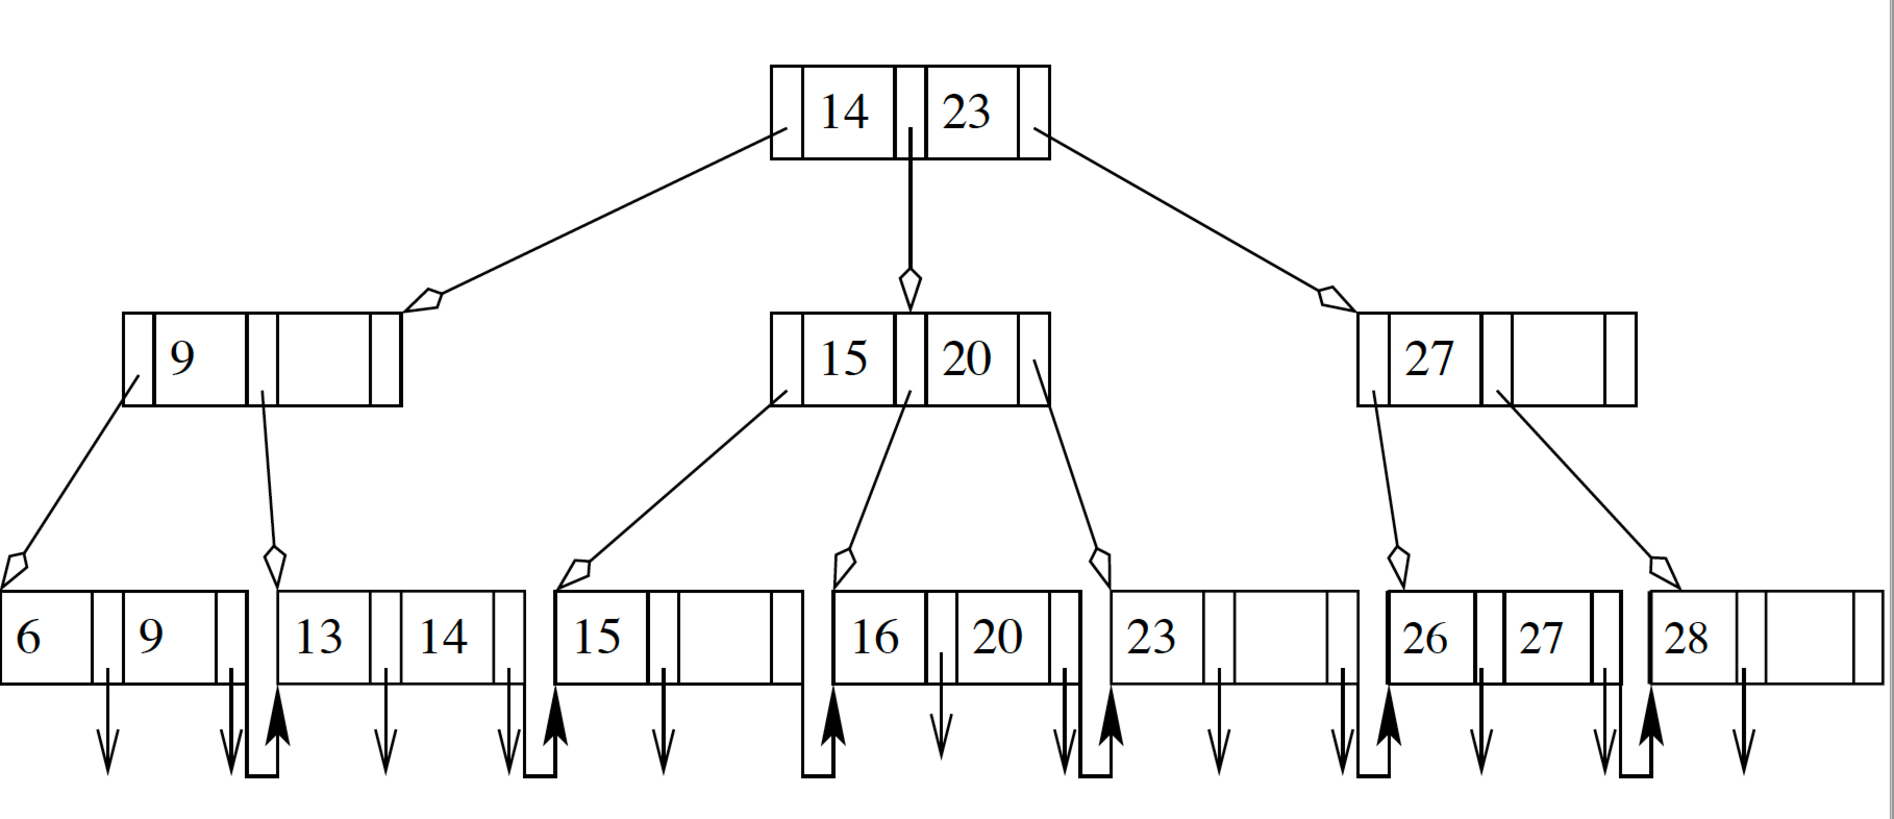
\includegraphics[scale=0.4]{../supports/figures/ex106-s1-hybride-20}}
    \caption{Un arbre B}  
    \label{arbreb}  
  \end{figure} 
  
%\fig{exm107}{Un arbre B+}

\begin{enumerate}
  
  \item Une table relationnelle contient 256\,500 lignes. 
   On la stocke dans une base avec des blocs
de 4\,000 octets. On 
suppose que chaque enregistrement a une taille de 
200 octets et que chaque bloc a un entête de 100 octets. 
Quel est le nombre d'enregistrements par bloc\,? Quel est le
  nombre de blocs nécessaire pour stocker la table
(on suppose que les blocs contiennent autant d'enregistrements
que possible)\,?

  \item Expliquez la différence entre un index dense et un
    index non-dense. Combien d'index denses peut-on construire
    sur un fichier\,? Combien d'index non-denses\,?

  \item La figure~\ref{arbreb} montre un arbre B. On peut stocker au plus 2 entrées par bloc.
         Indiquez le rôle
    des différents pointeurs représentés, et donnez l'arbre après
   insertion d'un enregistrement de clé 17 (dessinez au moins les parties
    de l'arbre qui ont changé).

  \item On effectue une recherche sur l'intervalle [13,23] (avant l'insertion
  de la clé 17). Combien
  de blocs lit-on dans l'index, et combien de blocs \emph{au pire} doit-on
  lire dans le fichier\,?

  \item On indexe une table par un arbre B sur un identifiant
    dont les valeurs sont fournies par une {\em séquence}. À 
   chaque insertion un compteur est incrémenté et fournit la valeur
        de clé de l'enregistrement inséré.

   On suppose qu'il n'y a que des insertions dans la table. Montrez
    que tous les n{\oe}uds de l'index qui ont un  frère droit
    sont exactement à moitié pleins.

\end{enumerate}

\begin{solution}
\begin{enumerate}
  \item On place 19 enregistrements par bloc.  Il faut 
        $\lceil \frac{256\,500}{19} \rceil = 13\,500$ blocs.

  \item Index dense et non dense: voir le cours
 
  \item Structure d'un arbre B+: voir le cours

   \item Au moment d'un éclatement, on se retrouve avec deux blocs
     remplis à moitié. Celui qui a un frère droit ne contient que
     valeurs de clés inférieures à celui de son frère droit.
     Comme on n'insère que des valeurs supérieures à toutes celles
     existantes, un n{\oe}ud qui a un frère droit ne sera jamais modifié.
\end{enumerate}
\end{solution}

%%%%%%%%%%%%%%%%%%%%%%%%

\section{Optimisation (9 points)}

Soit les tables relationnelles suivantes (les attributs qui forment 
une clé sont en gras):

\begin{itemize}
  \item Produit  (\textbf{code}, nom, marque, prix)
  \item Client  (\textbf{id}, nom, prénom)
  \item Achat    (\textbf{codeProduit}, \textbf{idClient}, date, quantité)
\end{itemize}


On donne ci-dessous une requête SQL et le plan d'exécution fourni par Oracle :

\begin{minted}{sql}
 select quantité
 from Produit as p, Client as c, Achat as a
 where p.code = a.codeProduit
 and   c.id = a.idClient
 and   prix > 50
\end{minted}

Plan d'exécution :


\begin{minted}[baselinestretch=.9,
               fontsize=\small,
               framesep=2mm]{text}
0 SELECT STATEMENT
  1 MERGE JOIN
    2 SORT JOIN
      3 NESTED LOOPS
        4 TABLE ACCESS FULL ACHAT
        5 TABLE ACCESS BY INDEX ROWID PRODUIT
          6 INDEX UNIQUE SCAN A34561
    7 SORT JOIN
      8 TABLE ACCESS FULL Client
\end{minted}

\begin{enumerate}
 \item Que peut-on déduire de ce plan\,: peut-on savoir s'il
    existe un index sur la table Client\,? 
   Sur la table Produit\,? Sur la table Achat\,? Si vous pensez
   qu'un index existe, donnez les attributs indexés. 
     Justifiez vos réponses.

\begin{solution}
Il existe un index sur l'attribut code de la table Produit;
en revanche pas d'index sur l'id de la table Client, sinon
on n'aurait  pas besoin d'un tri-fusion. Tout ce qu'on peut
dire sur la table Achat, c'est qu'il n'y a pas d'index dont
l'id du client soit un préfixe (sinon on pourrait parcourir séquentiellement
Client et accéder aux autres tables par l'index).
\end{solution}

  \item Quels sont les algorithmes de jointure utilisés? 
      Expliquer le fonctionnement de ce plan d'exécution.

\begin{solution}
Un algo. de boucles imbriquées indexées sur Achat-Produit, un
algo de sort/merge sur le résultat de cette jointure et la
table Client.
\end{solution}

  \item Quel(s) index  peut-on ajouter pour obtenir les meilleures
      performances possibles\,? Donnez, sous la forme 
      que vous souhaitez, le plan d'exécution
        après ajout d'index.

\begin{solution}
Solution : on peut ajouter un index sur l'id de client, et sur le
prix du produit. Dans ce cas le plan est:

\begin{minted}[baselinestretch=.9,
               fontsize=\small,
               framesep=2mm]{text}
Plan d'execution
--------------------------------------------------------------------------------
0 SELECT STATEMENT
  1 NESTED LOOPS
    2 NESTED LOOPS
      3 TABLE ACCESS BY INDEX ROWID PRODUIT
        4 INDEX RANGE SCAN PRODUIT_PRIX
      5 TABLE ACCESS BY INDEX ROWID ACHAT
        6 INDEX UNIQUE SCAN ACHAT_CODEPRODUIT
    7 TABLE ACCESS BY INDEX ROWID CLIENT
      8 INDEX RANGE SCAN CLIENT_ID
\end{minted}
\end{solution}

  \item On fait une jointure entre les tables Produit et Achat.
   Produit occupe 500 blocs, Achat 10\,000 blocs. Vaut-il mieux 
    appliquer un algorithme de boucles imbriquées ou de hachage
    si la mémoire $M$ disponibe est de $600$ blocs\,? 
    
    
   \item Même question si la mémoire est
        de 101 blocs? Indiquez dans chaque cas le nombre
    d'entrées/sorties (sans prendre en compte l'écriture du résultat final).

    Pour ces deux questions\,: expliquez le fonctionnement respectif 
    des boucles imbriquées et de la jointure par hachage.
    
\begin{solution}
$M=600$: on lit Produit en mémoire, et une lecture de Achat suffit,
dont coût égal à 10\,500 blocs pour les boucles imbriquées.
Avec le hachage: on hache Produit (coût = 1\,000 blocs)
et Achat (coût = 20\,000 blocs). On relit les deux. Coût
total\,: 31\,500 blocs.

$M=100$: avec les boucles imbriquées on doit lire 1 fois Produit et
5 fois Achat, pour un coût de 50\,500 blocs. Sinon on hache les
deux (coût= 21\,000 blocs) et on les relit une fois (coût total
31\,500 blocs). 
\end{solution}
\end{enumerate}


\section{Concurrence (4 points)}

Soit l'exécution concurrente suivante :

$$H = r_2[y] w_1[x] r_1[x] r_3[z] w_2[z] w_3[x] c_1 w_3[z] c_3 r_2[x] c_2$$

1. Donner la liste des conflits de $H$. (0,5 point)

\begin{solution}

Conflits:
\begin{enumerate}
 \item En $x$: $w_1w_3$, $w_1r_2$, $r_1w_3$, et $w_3r_2$
  \item En $y$: -
  \item En $z$: $r_3w_2$, $w_2w_3$
\end{enumerate}

\end{solution}

2. Donner le graphe de sérialisabilité de $H$. Que pouvez-vous déduire de ce graphe ? (0,5 point)

\begin{solution}
Les arêtes\,: $T_1 \to T_3$ ; $T_1 \to T_2$ ; $T_3 \to T_2$ ; $T_3 \to T_2$  et  $T_2 \to T_3$.

Il y a un cycle donc l'exécution n'est pas sérialisable.
\end{solution}

3. Donner l'exécution obtenue 
par application de l'algorithme de verrouillage à deux phases. 
Détailler le déroulement de l'algorithme. 
 (2 points)

\begin{solution}
La lecture $w_2[z]$ est bloquée par $r_3[z]$. $T_2$ est mise en attente et $T_3$ termine. $T_2$
est alors débloquée et termine.

$$H_{finale} = r_2[y] w_1[x] r_1[x] r_3[z] c_1 w_3[x] w_3[z] c_3 w_2[z] r_2[x] c_2$$
\end{solution}



